\documentclass[12pt]{article}
\usepackage[left=1cm, right=1cm, top=2cm,bottom=1.5cm]{geometry} 

\usepackage[parfill]{parskip}
\usepackage[utf8]{inputenc}
\usepackage[T2A]{fontenc}
\usepackage[russian]{babel}
\usepackage{enumitem}
\usepackage[normalem]{ulem}
\usepackage{amsfonts, amsmath, amsthm, amssymb, mathtools}
\usepackage{tabularx}
\usepackage{hhline}

\usepackage{accents}
\usepackage{fancyhdr}
\pagestyle{fancy}
\renewcommand{\headrulewidth}{1.5pt}
\renewcommand{\footrulewidth}{1pt}

\usepackage{graphicx}
\usepackage[figurename=Рис.]{caption}
\usepackage{subcaption}
\usepackage{float}

%%Наименование папки откуда забирать изображения
\graphicspath{ {./images/} }

%%Изменение формата для ввода доказательства
\renewcommand{\proofname}{$\square$  \nopunct}
\renewcommand\qedsymbol{$\blacksquare$}

%%Изменение отступа на таблицах
\addto\captionsrussian{%
	\renewcommand{\proofname}{$\square$ \nopunct}%
}
%% Римские цифры
\newcommand{\RN}[1]{%
	\textup{\uppercase\expandafter{\romannumeral#1}}%
}

%% Для удобства записи
\newcommand{\MR}{\mathbb{R}}
\newcommand{\MQ}{\mathbb{Q}}
\newcommand{\MN}{\mathbb{N}}
\newcommand{\MI}{\mathrm{I}}
\newcommand{\MJ}{\mathrm{J}}
\newcommand{\MH}{\mathrm{H}}
\newcommand{\MT}{\mathrm{T}}
\newcommand{\MU}{\mathcal{U}}
\newcommand{\MV}{\mathcal{V}}
\newcommand{\MW}{\mathcal{W}}
\newcommand{\VN}{\varnothing}
\newcommand{\VE}{\varepsilon}

\theoremstyle{definition}
\newtheorem{defn}{Опр:}
\newtheorem{rem}{Rm:}
\newtheorem{prop}{Утв.}
\newtheorem{exrc}{Упр.}
\newtheorem{lemma}{Лемма}
\newtheorem{theorem}{Теорема}
\newtheorem{corollary}{Следствие}

\newenvironment{cusdefn}[1]
{\renewcommand\thedefn{#1}\defn}
{\enddefn}

\DeclareRobustCommand{\divby}{%
	\mathrel{\text{\vbox{\baselineskip.65ex\lineskiplimit0pt\hbox{.}\hbox{.}\hbox{.}}}}%
}
%Короткий минус
\DeclareMathSymbol{\SMN}{\mathbin}{AMSa}{"39}
%Длинная шапка
\newcommand{\overbar}[1]{\mkern 1.5mu\overline{\mkern-1.5mu#1\mkern-1.5mu}\mkern 1.5mu}
%Функция знака
\DeclareMathOperator{\sgn}{sgn}

%Функция ранга
\DeclareMathOperator{\rk}{\text{rk}}

%Обозначение константы
\DeclareMathOperator{\const}{\text{const}}

%Интеграл в большом формате
\DeclareMathOperator{\dint}{\displaystyle\int}

\newcommand{\smallerrel}[1]{\mathrel{\mathpalette\smallerrelaux{#1}}}
\newcommand{\smallerrelaux}[2]{\raisebox{.1ex}{\scalebox{.75}{$#1#2$}}}

\newcommand{\smallin}{\smallerrel{\in}}
\newcommand{\smallnotin}{\smallerrel{\notin}}

\newcommand*{\medcap}{\mathbin{\scalebox{1.25}{\ensuremath{\cap}}}}%
\newcommand*{\medcup}{\mathbin{\scalebox{1.25}{\ensuremath{\cup}}}}%

\makeatletter
\newcommand{\vast}{\bBigg@{3.5}}
\newcommand{\Vast}{\bBigg@{5}}
\makeatother

%Скалярное произведение
\DeclarePairedDelimiterX{\inner}[2]{\langle}{\rangle}{#1, #2}

%Подпись символов снизу
\newcommand{\ubar}[1]{\underaccent{\bar}{#1}}

\begin{document}
\lhead{Математический анализ - \RN{2}}
\chead{Шапошников С.В.}
\rhead{Лекция - 20}
\section*{Условный экстремум}
Пусть $M^k$ - гладкая $k$-мерная поверхность в $\MR^n$. Пусть $f \colon \MR^n \to \MR$ - непрерывно дифференцируемая функция. 
\begin{defn}
	Точка $p \in M^k$ является \uwave{точкой локального условного максимума} функции $f$ на $M^k$, если: 
	$$
		\exists \, \MU(p) \colon \forall x \in \MU(p) \cap M^k, \, f(x) \leq f(p)
	$$
\end{defn}
\begin{defn}
	Точка $p \in M^k$ является \uwave{точкой строгого локального условного максимума} функции $f$ на $M^k$, если: 
	$$
		\exists \, \MU(p) \colon \forall x \in \MU(p) \cap M^k, x \neq p, \, f(x) < f(p)
	$$
\end{defn}
\begin{defn}
	Точка $p \in M^k$ является \uwave{точкой локального условного минимума} функции $f$ на $M^k$, если: 
	$$
		\exists \, \MU(p) \colon \forall x \in \MU(p) \cap M^k, \, f(x) \geq f(p)
	$$
\end{defn}
\begin{defn}
	Точка $p \in M^k$ является \uwave{точкой строгого локального условного минимума} функции $f$ на $M^k$, если: 
	$$
		\exists \, \MU(p) \colon \forall x \in \MU(p) \cap M^k, x \neq p, \, f(x) > f(p)
	$$
\end{defn}
\begin{defn}
	Точки локального условного максимума и минимума (в том числе строгого) называются \uwave{точками локального условного экстремума}.
\end{defn}
Таким образом, мы изучаем на экстремум функцию $f$, но смотрим не на всём $\MR^n$, а ограничиваемся значениями на $M^k$. Мы хотим научиться узнавать, чем характерны точки в которых функция $f$ достигает своего максимума и минимума на поверхности $M^k$. Всего два основных утверждения.
\subsection*{Необходимое условие локального условного экстремума}
\begin{theorem}\textbf{(Необходимое условие)}
	Если $p$ - точка локального условного экстремума на $M^k$, то: 
	$$
		\nabla f(p) \perp T_p M^k
	$$
	В частности, если градиент $\nabla f(p) \neq 0$, то $T_p M^k \subset TS$, где $TS$ это  касательное пространство в точке $p$ к $\{x \colon f(x) = f(p)\}$.
\end{theorem}
\begin{figure}[H]
	\centering
	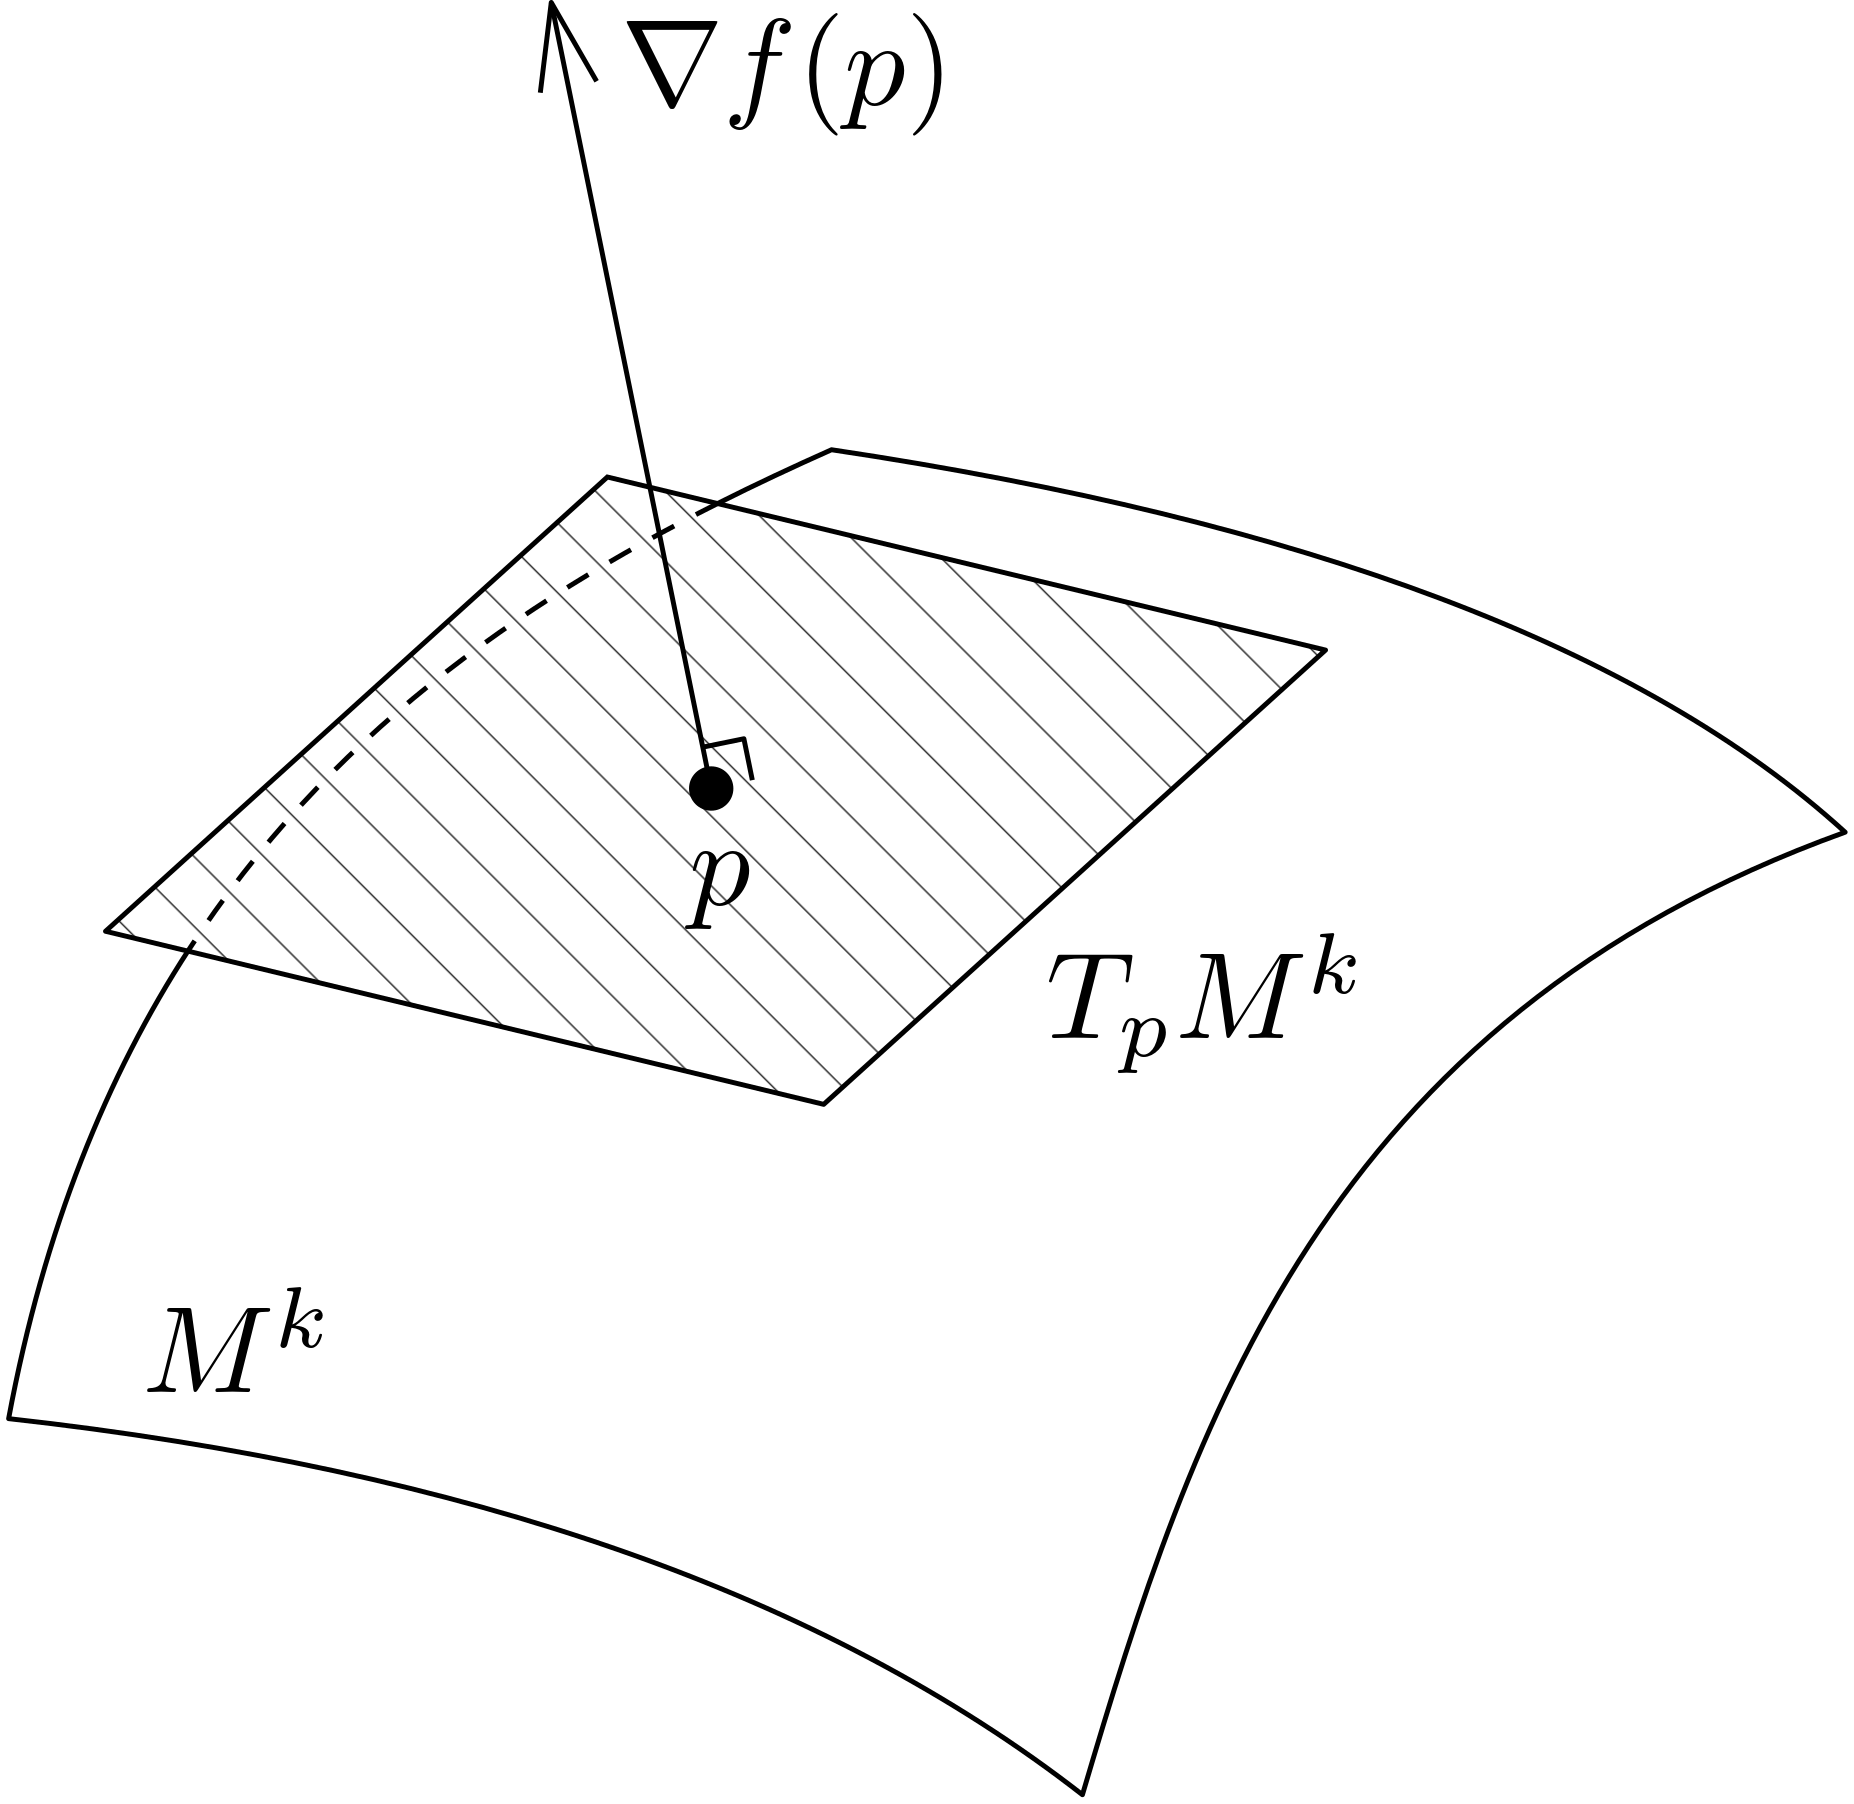
\includegraphics[width=0.3\textwidth]{20_1.png}
	\caption{Градиент функции $f$ в точке $p$ перпендикулярен касательной плоскости.}
	\label{20_1}
\end{figure}
\textbf{\uline{Идея}}: Если в точке $p$  у функции $f$ локальный условный экстремум и мы в ней посчитаем градиент, то он должен быть перпендикулярен поверхности $M^k \Rightarrow$ перпендикулярен касательной плоскости. 

С другой стороны, градиент (невырожденный) это то что перпендикулярно множеству уровня. Если градиент $f$ отличен от нуля, то в окрестности точки $p$ множество уровня $\{x \colon f(x) = f(p)\}$ является гладкой $(n-1)$-мерной поверхностью и тогда свойства перпендикулярности означают, что касательная плоскость $T_p M^k$ лежит среди всех касательных векторов $TS\big(f(p)\big)$ уровня $f(x) = f(p)$.
\begin{figure}[H]
	\centering
	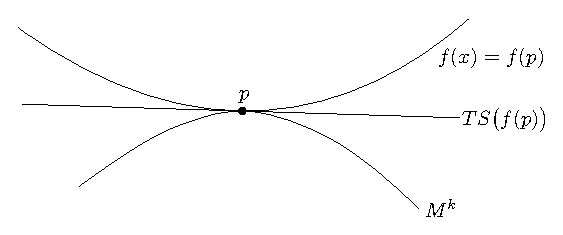
\includegraphics[width=0.55\textwidth]{20_2.eps}
	\caption{Касательная плоскость $T_p M^k$ к $M^k$ в $p$ содержится внутри касательного пространства $TS\big(f(p)\big)$.}
	\label{20_2}
\end{figure}
\textbf{\uline{Геометрический смысл}}: Если размерность $TS\big(f(p)\big)$ и $T_p M^k$ была бы одинаковая, то они бы совпадали $\Leftrightarrow$ происходит касание между поверхностями $M^k$ и $\{x \colon f(x) = f(p)\}$. Но если размерность $T_p M^k$ меньше размерности $TS\big(f(p)\big)$ (множество уровня функции $f$ это гиперповерхность, а  поверхность с условиями $M^k$ уже меньшей размерности), то касательное пространство к $M^k$ будет содержаться в касательном пространстве к множеству уровня.

Пусть мы в $\MR^3$, можно поставить два дополнительных условия (два уравнения) и взять поверхность $M^k$ в виде линий. Пусть $M^k$ это линия $\Rightarrow k = 1$. Если на этой линии функция $f$ достигает экстремума в точке $p$, то касательный вектор в этой точке к этой линии должен лежать в касательном пространстве к множеству уровня функции $f$.

\begin{figure}[H]
	\centering
	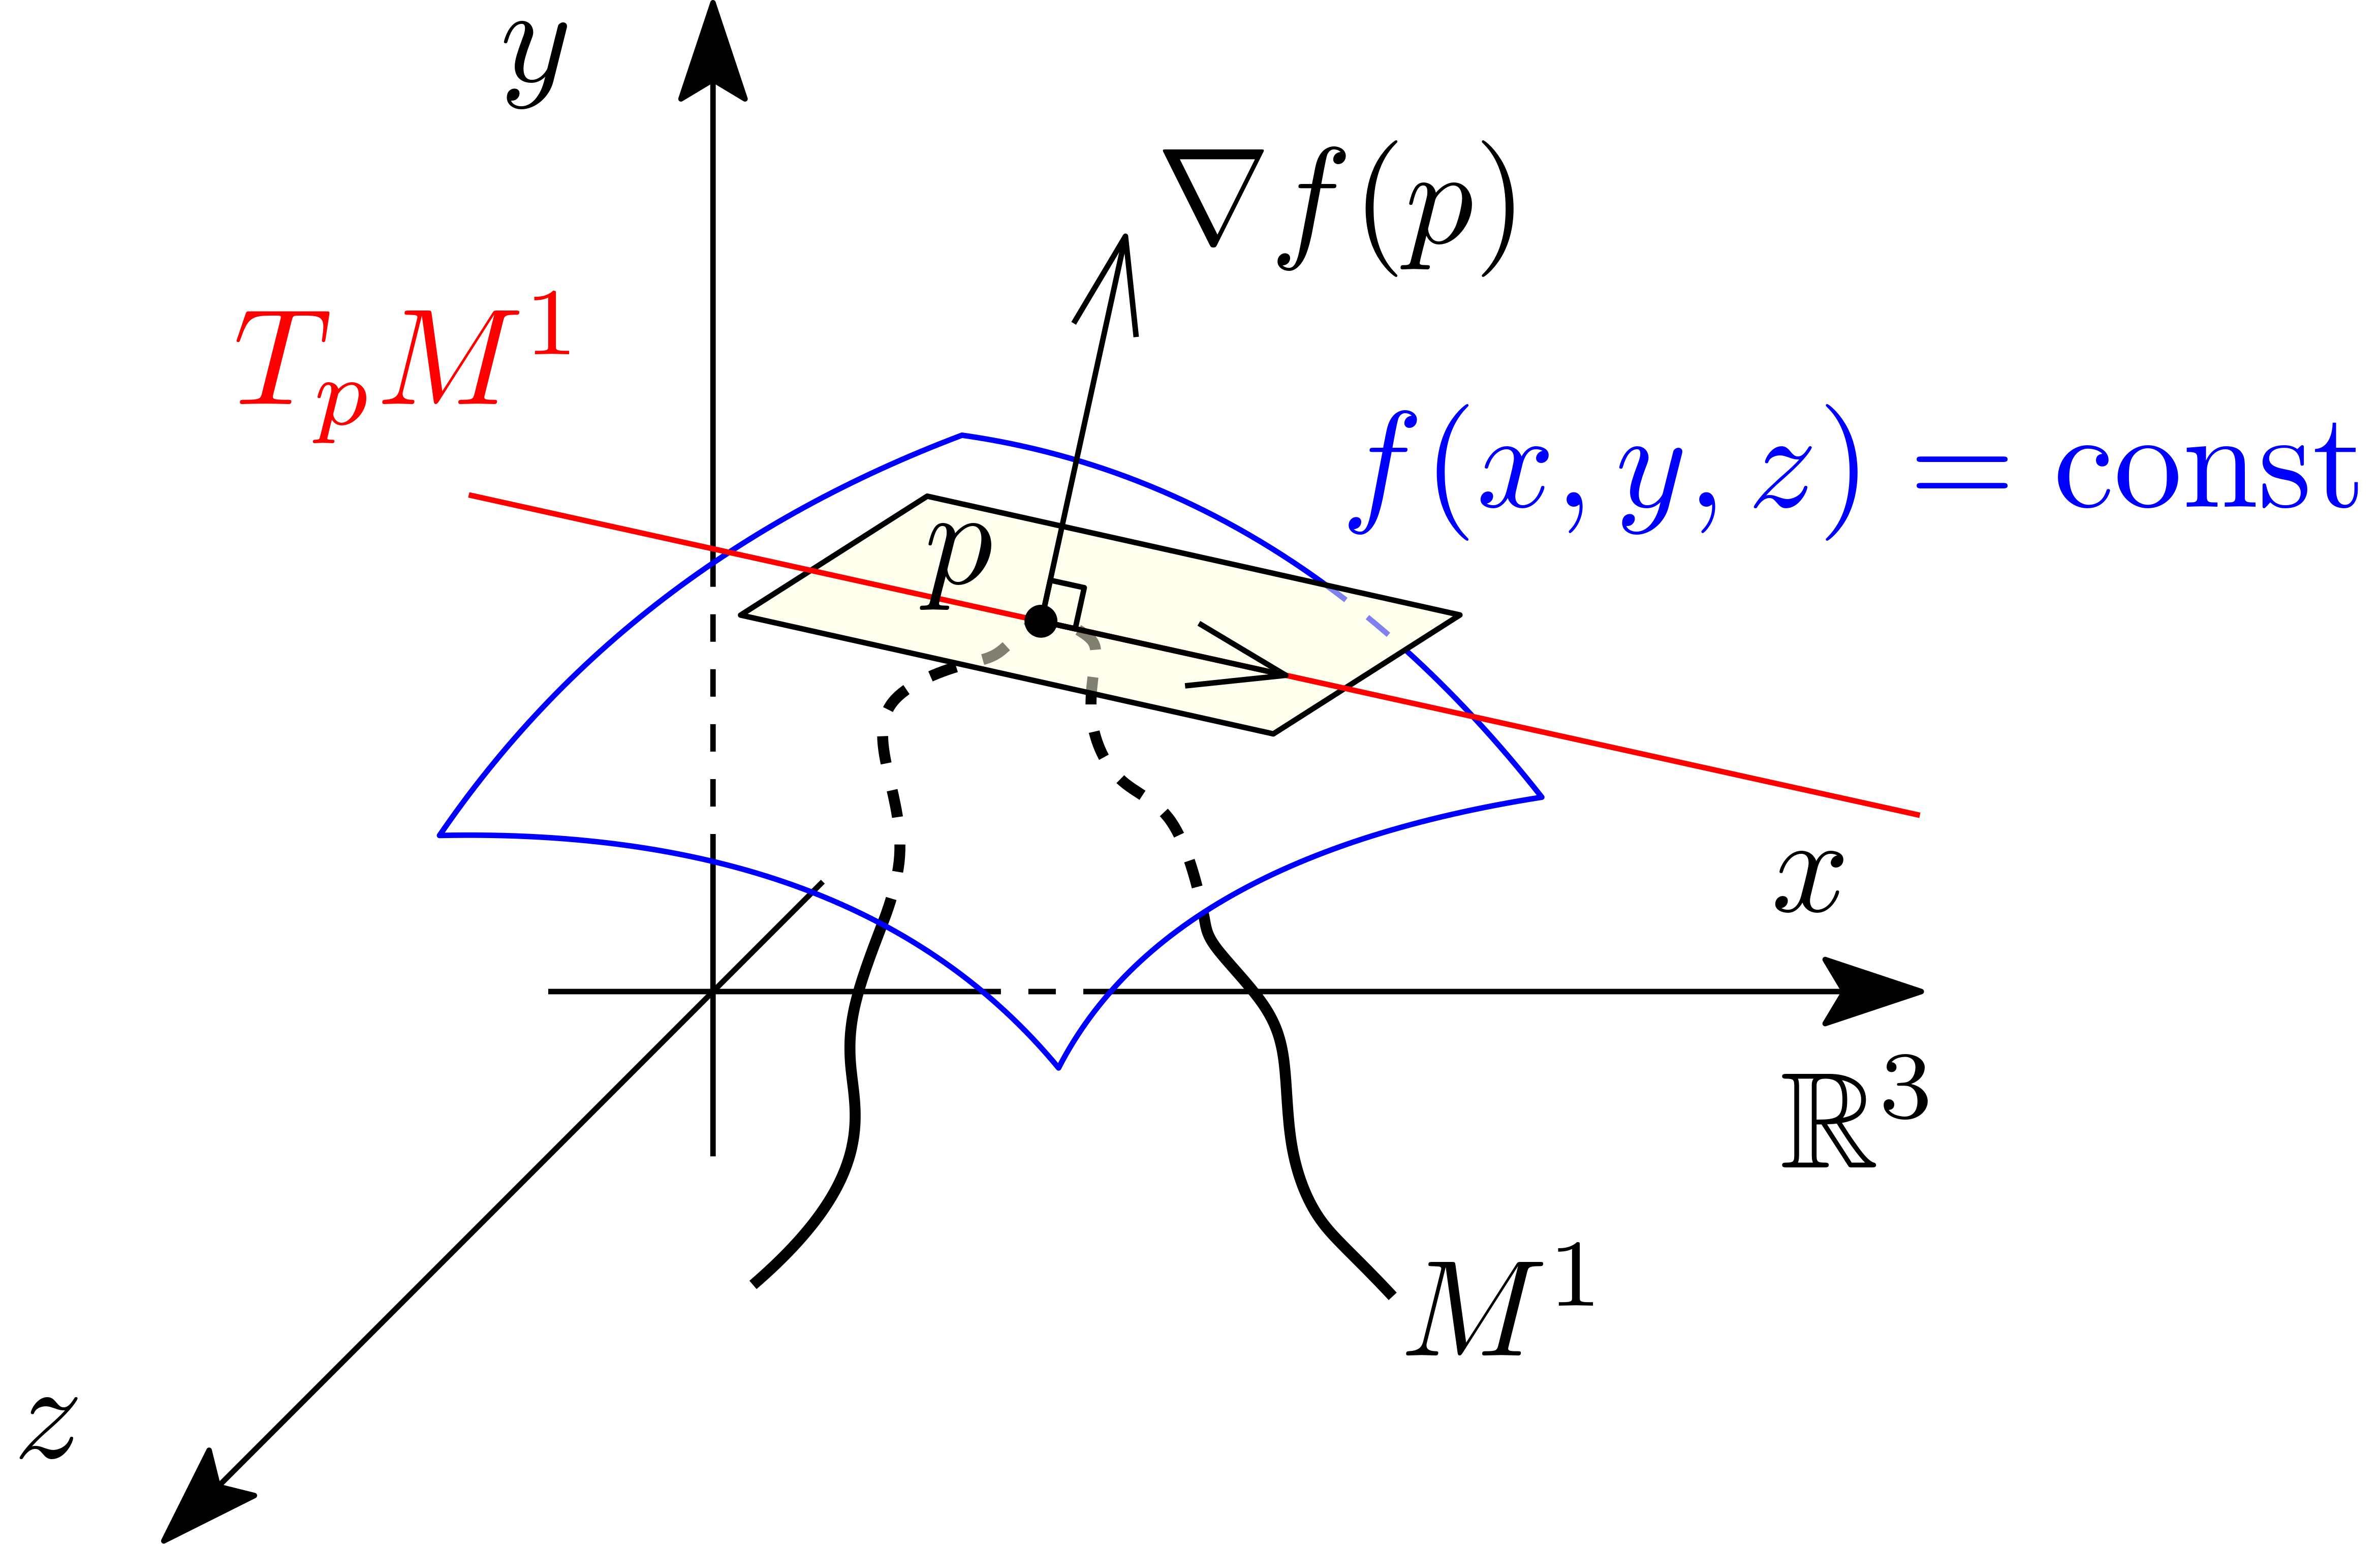
\includegraphics[width=0.45\textwidth]{20_3.png}
	\caption{Касательная плоскость к $M^1 \subset$ касательная плоскость к линии уровня $f(p)$.}
	\label{20_3}
\end{figure}
\begin{rem}
	Это воплощение геометрического образа, которое мы видели на конкретных примерах по поиску условного экстремума в предыдущих лекциях.
\end{rem}
\begin{proof}
	Пусть $v \in T_p M^k \Rightarrow \exists \, \gamma \colon \gamma(0) = p, \, \gamma(t) \in M^k, \, \dot{\gamma}(0) = v$. Рассмотрим $f\big(\gamma(t)\big)$ - функция одного аргумента, у которой в точке $t = 0$ - локальный экстремум, поскольку у функции $f$ в точке $p$ - локальный экстремум.
	\begin{figure}[H]
		\centering
		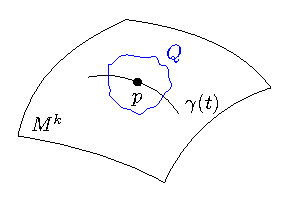
\includegraphics[width=0.3\textwidth]{20_4.eps}
		\caption{В окрестности $Q$ точки $p$, функция $f$ имеет точку экстремума в $p$.}
		\label{20_4}
	\end{figure}
	Поскольку функция одномерная, то в точке $t = 0$ верно следующее:
	$$
		\dfrac{d}{dt}\bigg|_{t=0}f\big(\gamma(t)\big) = 0 \Rightarrow \langle \nabla f(p), \dot{\gamma}(0) \rangle = 0 \Rightarrow \langle \nabla f(p), v \rangle = 0 \Rightarrow \nabla f(p) \perp T_p M^k
	$$
\end{proof}
\begin{corollary}
	Если в условиях теоремы множество $M^k$ в окрестности точки $p$ задано системой уравнений: $F_{k+1}(x) = 0, \dotsc, F_n(x) = 0$, где градиенты $\nabla F_{k+1}(p), \dotsc, \nabla F_n (p)$ - линейно независимы, то: 
	$$
		\exists \, \lambda_{k+1}, \dotsc, \lambda_n \in \MR \colon \nabla f(p) = \lambda_{k+1} \nabla F_{k+1} (p) + \dotsc + \lambda_n \nabla F_n(p)
	$$
\end{corollary}
\begin{proof}
	По утверждению с прошлой лекции: 
	$$
		v \in T_pM^k \Leftrightarrow 
		\left\{
		\begin{array}{ccc}
			\langle \nabla F_{k+1}(p),v \rangle & =& 0\\
			\vdots & \vdots & \vdots \\
			\langle \nabla F_n(p),v \rangle &=& 0
		\end{array}
		\right.
		\Leftrightarrow 
		\left\{
		\begin{array}{c}
			v \perp \nabla F_{k+1}(p)\\
			\vdots  \\
			v \perp \nabla F_n(p)
		\end{array}
		\right.
	$$
	Заметим, что $\dim{(T_pM^k)} = k$, число градиентов равно $(n-k)$, они линейно независимы и лежат в ортогональной плоскости $(T_pM^k)^{\perp}$. Из линейной алгебры мы знаем, что размерность ортогонального пространства равна $\dim{(\MR^n)} - \dim{(T_pM^k)} = n -k$, значит $\nabla F_{k+1}(p), \dotsc, \nabla F_n(p)$ - это базис в $(T_pM^k)^{\perp}$.
	\begin{figure}[H]
		\centering
		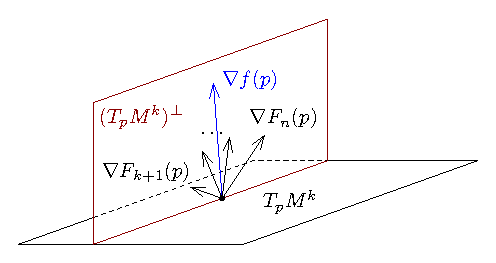
\includegraphics[width=0.45\textwidth]{20_5.eps}
		\caption{Ортогональное пространство $(T_pM^k)^{\perp}$.}
		\label{20_5}
	\end{figure}
	Поскольку $\nabla f(p) \perp T_pM^k \Rightarrow \nabla f(p) \in (T_pM^k)^{\perp} \Rightarrow \nabla f(p)$ является линейной комбинацией базисных векторов ортогонального пространства $\Rightarrow\exists \, \lambda_{k+1}, \dotsc, \lambda_n \in \MR \colon \nabla f(p) = \lambda_{k+1} \nabla F_{k+1} (p) + \dotsc + \lambda_n \nabla F_n(p)$.
\end{proof}
\subsection*{Стандартная задача на условный экстремум}
В обычной постановке задачи звучат так:
$$
	\left\{
	\begin{array}{c}
		f \to \text{extr}!\\
		F_{k+1} = 0 \\
		\vdots \\
		F_n = 0	
	\end{array}
	\right.
$$
где условия $F_{k+1} = 0, \dotsc, F_n = 0$ задают $k$-мерную поверхность. Нарисуем в точке $p$ касательную плоскость, тогда градиенты $\nabla F_{k+1}(p), \dotsc, \nabla F_n(p)$ будут лежать в ортогональном дополнении и градиент функции $f$ в точке $p$ перпендикулярен касательному пространству. 
\begin{figure}[H]
	\centering
	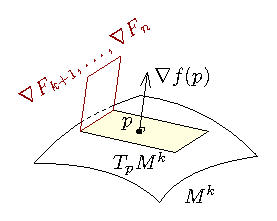
\includegraphics[width=0.3\textwidth]{20_6.eps}
	\caption{Градиент функции $f$ выражается через градиенты $\nabla  F_{k+1}, \dotsc, \nabla F_n$.}
	\label{20_6}
\end{figure}
Следовательно $\nabla f(p)$ должен выражаться через градиенты  $\nabla F_{k+1}(p), \dotsc, \nabla F_n(p)$, то есть:
$$
	\nabla f(p) = \lambda_{k+1} \nabla F_{k+1} (p) + \dotsc + \lambda_n \nabla F_n(p)
$$
\subsection*{Метод множителей Лагранжа}
Поиск условного экстремума можно представить в ином виде. Запишем \uwave{функцию Лагранжа}:
$$
	L(x,\lambda) =f(x) - \lambda_{k+1} F_{k+1}(x) - \dotsc - \lambda_n F_n(x)
$$
\textbf{\uline{Необходимое условие условного экстремума}}:
$$
	\left\{
		\renewcommand\arraystretch{2}
		\begin{array}{ccl}
			\dfrac{\partial L}{\partial x_i} & = & 0, \, i = \overline{1, n}\\
			\dfrac{\partial L}{\partial \lambda_j} & = & 0, \, j = \overline{k+1,n}
		\end{array}
	\right.
$$
где первые равенства получены из теоремы о достаточном признаке:
$$
	\dfrac{\partial L}{\partial x_i}  =  0, \, i = \overline{1, n} \Leftrightarrow \nabla f(p) - \lambda_{k+1} \nabla F_{k+1} (p) - \dotsc - \lambda_n \nabla F_n(p) = 0
$$
и вторые равенства есть просто задание $k$-мерной поверхности:
$$
	\dfrac{\partial L}{\partial \lambda_j} =  0, \, j = \overline{k+1,n} \Leftrightarrow F_j(x) = 0, \, j = \overline{k+1,n}
$$

\textbf{Cуть метода}: хотим исследовать функцию $f$ на экстремум при условии $F_{k+1} = 0,\dotsc, F_n = 0$, тогда необходимо составить функцию Лагранжа и действовать также как и раньше, исследуя функцию на обычный экстремум. Конкретнее, если хотим найти точки подозрительные на экстремум, то необходимо приравнять частные производные функции Лагранжа к нулю.

\textbf{Задача Лагранжа}: Пусть есть тонкая проволока, которая задается как $F(x) = 0$ и по ней без трения двигается бусина под действием некоей силы. Сила потенциальна (то есть она тянет куда-то бусину) и задается как $\nabla f$. Изучаются точки равновесия, то есть точки в которых эта бусина будет в покое на заданной кривой.
\begin{figure}[H]
	\centering
	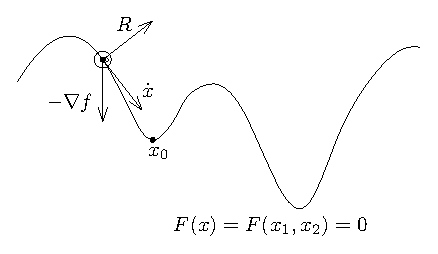
\includegraphics[width=0.45\textwidth]{20_7.eps}
	\caption{Задача Лагранжа: ищем точки равновесия бусины на проволоке.}
	\label{20_7}
\end{figure}
Движение бусины описывается следующим образом (по закону Ньютона): $\ddot{x} = - \nabla f + R$ (массу бусины считаем равной $1$). Домножим на $\dot{x}$ (вектор скорости: всегда будет направлен по касательной к этой проволоке $\Rightarrow$ будет перпендикулярен силе рекции опоры $R$), тогда получим:
$$
	\langle \ddot{x}, \dot{x} \rangle = -\langle \nabla f, \dot{x} \rangle + \langle R, \dot{x} \rangle =  -\langle \nabla f, \dot{x} \rangle \Leftrightarrow \dfrac{d}{dt}\bigg(\dfrac{\|\dot{x}\|^2}{2}\bigg) = -\dfrac{d}{dt}f \big(x(t)\big)
$$
Получаем закон сохранения энергии:
$$
	\dfrac{\|\dot{x}\|^2}{2} + f(x) = \const 
$$
Представим, что взяли точку минимума потенциальной энергии $x_0$ ($f(x)$ трактуется как потенциальная энергия). Может ли бусина уехать из этой точки? Нет, так как необходима положительная скорость для этого $\Rightarrow$ необходимо уменьшить $f$, чтобы сумма оставалась константой, но мы и так взяли минимум. Точка минимума является точкой равновесия для бусины, а это означает что силы должны быть равны:
$$
	-\nabla f(x_0) + R(x_0) = 0
$$
Сила реакции опоры действует перпендикулярно линии $F(x) = 0 \Rightarrow R = \lambda \nabla F$ и получим:
$$
	\nabla f(x_0) = \lambda \nabla F(x_0)
$$

\newpage
\subsection*{Достаточное условие локального условного экстремума}
\begin{theorem}\textbf{(Достаточное условие)}
	Пусть поверхность $M^k$ в окрестности точки $p$ задана системой уравнений $F_{k+1} = 0, \dotsc, F_n = 0$, где $F_i$ - дважды непрерывно дифференцируемые функции, $f$ тоже дважды непрерывно дифференцируемая функция и в точке $p$ выполняется необходимое условие локального условного экстремума. Пусть $L(x,\lambda) = L(x)$ - это соответствующая функция Лагранжа. Тогда:
	\begin{enumerate}[label ={\arabic*)}]
		\item Если $d^2 L(p, h) > 0, \, \forall h \neq 0, \, h \in T_p M^k$, то $p$ - точка строгого локального условного минимума функции $f$;
		\item Если $d^2 L(p, h) < 0, \, \forall h \neq 0, \, h \in T_p M^k$, то $p$ - точка строгого локального условного максимума функции $f$;
		\item Если $\exists \, v,h \in T_p M^k \colon d^2 L(p,v) > 0, \, d^2 L(p,h) < 0$, то $p$ не является точкой локального условного экстремума;
	\end{enumerate}
\end{theorem}

\begin{rem}
	Проверять положительную или отрицательную определенность необходимо не на всех векторах, а только на касательных пространствах. 
	
	В точке $p$ знак приращения функции определяется вторым дифференциалом, но приращения функции надо брать вдоль заданной поверхности $M^k$, а это все равно что взять касательные приращения (брать только касательные вектора). И таким образом, мы смотрим как меняется функция вдоль касательных направлений.
\end{rem}
\begin{rem}
	Отметим также, что для изучения свойств $f$ мы рассматриваем новую функцию $L$. Почему так? Почему бы не использовать достаточные условия локального экстремума:
	$$
		f(p+h) - f(p) = \langle \nabla f(p), h\rangle + \tfrac{1}{2}d^2f(p,h) + \dotsc
	$$
	Пусть $h \in T_p M^k$, тогда:
	$$
		f(p + h) - f(p) = 0 + + \tfrac{1}{2}d^2f(p,h) + \dotsc
	$$
	Почему так нельзя? Так нельзя поскольку $p + h \notin M^k$. Из-за того, что поверхность это нелинейный объект и приходится переходить к функции Лагранжа. Ровно по этой же причине второй дифференциал не является инвариантным при замене координат.
\end{rem}
\begin{proof}
	Выпишем функцию Лагранжа $L(x)$:
	$$
		L(x) = L(x,\lambda) =f(x) - \lambda_{k+1} F_{k+1}(x) - \dotsc - \lambda_n F_n(x)
	$$
	и заметим что на $M^k$ верно $f(x) = L(x)$, поскольку если $x \in M^k \Rightarrow F_{k+1}(x) = 0, \dotsc, F_n(x) = 0$. Следовательно $p$ - точка экстремума $L$ на $M^k \Leftrightarrow p$ - точка экстремума $f$ на $M^k$. Заметим также, что:
	$$
		\dfrac{\partial L}{\partial x_i}(p) = 0, \, i = \overline{1,n}
	$$
	из необходимого условия локального условного экстремума.
	
	Мы ранее обсуждали, что поверхность $M^k$ в окрестности точки $p$ можно задать параметрически:
	$$
		\left\{
			\begin{array}{ccc}
				x_1& = &x_1(u_1,\dotsc, u_k) \\
				\vdots & \vdots & \vdots \\
				x_n& = &x_n(u_1,\dotsc, u_k)
			\end{array}
		\right.
	$$
	где $u_1,\dotsc, u_k$ находятся в окрестности нуля $W$ и $x(0) = p$. Обозначим $L\big(x(u)\big) = H(u)$. Точка $p$ - точка локального экстремума $L$ на $M^k \Leftrightarrow u = 0$ - точка локального экстремума $H$.
	
	Таким образом, задача о локальном условном экстремуме свелась к задаче об обычном локальном экстремуме функции $H$ в координатах $u_1, \dotsc, u_k$. Рассмотрим следующее:
	$$
		\dfrac{\partial H}{\partial u_m}(0) = \sum\limits_{i} \dfrac{\partial L}{\partial x_i}(p){\cdot}\dfrac{\partial x_i}{\partial u_m}(0)  = \sum\limits_{i} 0 {\cdot}\dfrac{\partial x_i}{\partial u_m}(0) = 0
	$$
	Следовательно для $H$ выполнено необходимое условие. Рассмотрим вторые производные $H$:
	$$
		\dfrac{\partial^2 H}{\partial u_l \partial u_m}(u) = \sum\limits_{j,i}\dfrac{\partial^2 L}{\partial x_j \partial x_i}\big(x(u)\big){\cdot}\dfrac{\partial x_j}{\partial u_l}(u){\cdot}\dfrac{\partial x_i}{\partial u_m}(u) + \sum\limits_{i} \dfrac{\partial L}{\partial x_i}\big(x(u)\big){\cdot}\dfrac{\partial^2 x_i}{\partial u_l \partial u_m}(u)
	$$
	Тогда в точке $0$ мы получим:
	$$
		\dfrac{\partial^2 H}{\partial u_l \partial u_m}(0) = \sum\limits_{j,i}\dfrac{\partial^2 L}{\partial x_j \partial x_i}\big(p\big){\cdot}\dfrac{\partial x_j}{\partial u_l}(0){\cdot}\dfrac{\partial x_i}{\partial u_m}(0) + 0 = \sum\limits_{j,i}\dfrac{\partial^2 L}{\partial x_j \partial x_i}\big(p\big){\cdot}\dfrac{\partial x_j}{\partial u_l}(0){\cdot}\dfrac{\partial x_i}{\partial u_m}(0)
	$$
	\begin{rem}
		Обычно про такой эффект говорят, что в критической точке второй дифференциал инвариантен.
	\end{rem}
	Запишем тогда второй дифференциал функции $H$:
	$$
		d^2 H(0,v) = \sum\limits_{j,i}\dfrac{\partial^2 L}{\partial x_i \partial x_j}(p){\cdot}\sum\limits_{l,m}\dfrac{\partial x_i}{\partial u_m}{\cdot}\dfrac{\partial x_j}{\partial u_l}{\cdot}v_m{\cdot}v_l = d^2L(p,h), \, h = \dfrac{\partial x}{\partial u_1}{\cdot}v_1 + \dotsc + \dfrac{\partial x}{\partial u_k}{\cdot}v_k
	$$
	где из предыдущей лекции мы знаем, что касательное пространство натянуто на вектора $\tfrac{\partial x}{\partial u_1}, \dotsc, \tfrac{\partial x}{\partial u_k}$. Следовательно верно, что: 
	$$
		h = \dfrac{\partial x}{\partial u_1}{\cdot}v_1 + \dotsc + \dfrac{\partial x}{\partial u_k}{\cdot}v_k \in T_p M^k, \, \forall v_l
	$$
	Таким образом, $d^2H(0,v) > 0 \Leftrightarrow d^2L(p,h) > 0$ и $d^2H(0,v) < 0 \Leftrightarrow d^2L(p,h) < 0$. Тем самым, утверждение вытекает из обычной теоремы о локальном экстремуме применяемой к функции $H$.
\end{proof}

\textbf{Пример}: Пусть на плоскости задана функция $f(x,y)$, необходимо найти её экстремум на оси $x$:
$$
	\left\{
	\begin{array}{l}
		f \to \text{extr}!\\
		y = 0
	\end{array}
	\right.
$$
Что в этом случае делаем? Подставляем $y=0$ и исследуем функцию $f(x,0)$.

В последнем шаге доказательства мы делаем нечто похожее: исследуем на экстремумы функцию $L$ на поверхности. Поверхность задана параметрически через $u_1, \dotsc, u_n$. Соответственно мы переводим функцию $L$ в функцию $H(u) = L\big(x(u)\big)$ и задача свелась к обычной задаче локального экстремума. 

Можно было поступить аналогично и с функцией $f \Rightarrow$ получить функцию $f\big(x(u)\big)$, но проблема будет в том, что мы не знаем что из себя представляет второй дифференциал ($d_u^2 f$) такой функции, так как там будут вторые производные координатных отображений (опять же наглядная демонстрация неинвариантности второго дифференциала). 

Поэтому использование функции $L$ с заменой координат дает нужный результат, поскольку есть понимание что $d^2_x L = d^2_u L$.

\end{document}